% Options for packages loaded elsewhere
\PassOptionsToPackage{unicode}{hyperref}
\PassOptionsToPackage{hyphens}{url}
\PassOptionsToPackage{dvipsnames,svgnames,x11names}{xcolor}
%
\documentclass[
  letterpaper,
  DIV=11,
  numbers=noendperiod]{scrartcl}

\usepackage{amsmath,amssymb}
\usepackage{iftex}
\ifPDFTeX
  \usepackage[T1]{fontenc}
  \usepackage[utf8]{inputenc}
  \usepackage{textcomp} % provide euro and other symbols
\else % if luatex or xetex
  \usepackage{unicode-math}
  \defaultfontfeatures{Scale=MatchLowercase}
  \defaultfontfeatures[\rmfamily]{Ligatures=TeX,Scale=1}
\fi
\usepackage{lmodern}
\ifPDFTeX\else  
    % xetex/luatex font selection
\fi
% Use upquote if available, for straight quotes in verbatim environments
\IfFileExists{upquote.sty}{\usepackage{upquote}}{}
\IfFileExists{microtype.sty}{% use microtype if available
  \usepackage[]{microtype}
  \UseMicrotypeSet[protrusion]{basicmath} % disable protrusion for tt fonts
}{}
\makeatletter
\@ifundefined{KOMAClassName}{% if non-KOMA class
  \IfFileExists{parskip.sty}{%
    \usepackage{parskip}
  }{% else
    \setlength{\parindent}{0pt}
    \setlength{\parskip}{6pt plus 2pt minus 1pt}}
}{% if KOMA class
  \KOMAoptions{parskip=half}}
\makeatother
\usepackage{xcolor}
\setlength{\emergencystretch}{3em} % prevent overfull lines
\setcounter{secnumdepth}{-\maxdimen} % remove section numbering
% Make \paragraph and \subparagraph free-standing
\ifx\paragraph\undefined\else
  \let\oldparagraph\paragraph
  \renewcommand{\paragraph}[1]{\oldparagraph{#1}\mbox{}}
\fi
\ifx\subparagraph\undefined\else
  \let\oldsubparagraph\subparagraph
  \renewcommand{\subparagraph}[1]{\oldsubparagraph{#1}\mbox{}}
\fi


\providecommand{\tightlist}{%
  \setlength{\itemsep}{0pt}\setlength{\parskip}{0pt}}\usepackage{longtable,booktabs,array}
\usepackage{calc} % for calculating minipage widths
% Correct order of tables after \paragraph or \subparagraph
\usepackage{etoolbox}
\makeatletter
\patchcmd\longtable{\par}{\if@noskipsec\mbox{}\fi\par}{}{}
\makeatother
% Allow footnotes in longtable head/foot
\IfFileExists{footnotehyper.sty}{\usepackage{footnotehyper}}{\usepackage{footnote}}
\makesavenoteenv{longtable}
\usepackage{graphicx}
\makeatletter
\def\maxwidth{\ifdim\Gin@nat@width>\linewidth\linewidth\else\Gin@nat@width\fi}
\def\maxheight{\ifdim\Gin@nat@height>\textheight\textheight\else\Gin@nat@height\fi}
\makeatother
% Scale images if necessary, so that they will not overflow the page
% margins by default, and it is still possible to overwrite the defaults
% using explicit options in \includegraphics[width, height, ...]{}
\setkeys{Gin}{width=\maxwidth,height=\maxheight,keepaspectratio}
% Set default figure placement to htbp
\makeatletter
\def\fps@figure{htbp}
\makeatother

\KOMAoption{captions}{tableheading}
\makeatletter
\makeatother
\makeatletter
\makeatother
\makeatletter
\@ifpackageloaded{caption}{}{\usepackage{caption}}
\AtBeginDocument{%
\ifdefined\contentsname
  \renewcommand*\contentsname{Table of contents}
\else
  \newcommand\contentsname{Table of contents}
\fi
\ifdefined\listfigurename
  \renewcommand*\listfigurename{List of Figures}
\else
  \newcommand\listfigurename{List of Figures}
\fi
\ifdefined\listtablename
  \renewcommand*\listtablename{List of Tables}
\else
  \newcommand\listtablename{List of Tables}
\fi
\ifdefined\figurename
  \renewcommand*\figurename{Figure}
\else
  \newcommand\figurename{Figure}
\fi
\ifdefined\tablename
  \renewcommand*\tablename{Table}
\else
  \newcommand\tablename{Table}
\fi
}
\@ifpackageloaded{float}{}{\usepackage{float}}
\floatstyle{ruled}
\@ifundefined{c@chapter}{\newfloat{codelisting}{h}{lop}}{\newfloat{codelisting}{h}{lop}[chapter]}
\floatname{codelisting}{Listing}
\newcommand*\listoflistings{\listof{codelisting}{List of Listings}}
\makeatother
\makeatletter
\@ifpackageloaded{caption}{}{\usepackage{caption}}
\@ifpackageloaded{subcaption}{}{\usepackage{subcaption}}
\makeatother
\makeatletter
\@ifpackageloaded{tcolorbox}{}{\usepackage[skins,breakable]{tcolorbox}}
\makeatother
\makeatletter
\@ifundefined{shadecolor}{\definecolor{shadecolor}{rgb}{.97, .97, .97}}
\makeatother
\makeatletter
\makeatother
\makeatletter
\makeatother
\ifLuaTeX
  \usepackage{selnolig}  % disable illegal ligatures
\fi
\IfFileExists{bookmark.sty}{\usepackage{bookmark}}{\usepackage{hyperref}}
\IfFileExists{xurl.sty}{\usepackage{xurl}}{} % add URL line breaks if available
\urlstyle{same} % disable monospaced font for URLs
\hypersetup{
  pdftitle={Fed's Forward Guidance},
  pdfauthor={Moustafa Chatzouz},
  colorlinks=true,
  linkcolor={blue},
  filecolor={Maroon},
  citecolor={Blue},
  urlcolor={Blue},
  pdfcreator={LaTeX via pandoc}}

\title{Fed's Forward Guidance}
\usepackage{etoolbox}
\makeatletter
\providecommand{\subtitle}[1]{% add subtitle to \maketitle
  \apptocmd{\@title}{\par {\large #1 \par}}{}{}
}
\makeatother
\subtitle{\emph{Some Stylised Facts and recent performance}}
\author{Moustafa Chatzouz}
\date{2023-04-28}

\begin{document}
\maketitle
\ifdefined\Shaded\renewenvironment{Shaded}{\begin{tcolorbox}[boxrule=0pt, interior hidden, enhanced, breakable, frame hidden, borderline west={3pt}{0pt}{shadecolor}, sharp corners]}{\end{tcolorbox}}\fi

\renewcommand*\contentsname{Table of contents}
{
\hypersetup{linkcolor=}
\setcounter{tocdepth}{3}
\tableofcontents
}
\begin{quote}
\begin{itemize}
\tightlist
\item
  \emph{Over the past two years, the Federal Reserve has been criticized
  by a wide range of actors - including the International Monetary Fund
  (IMF), financial markets, top academic economists, and even its own
  top officials - for being too slow to act on inflation and maintaining
  a monetary policy stance that is too loose given record high
  inflation. However, many of these arguments still rely on backward
  looking measures, such as the distance of policy rate from neutral, as
  well as on ``old-school'' thinking that implicitly ignores how much of
  an impact forward guidance can have.}
\end{itemize}
\end{quote}

\begin{quote}
\begin{itemize}
\tightlist
\item
  \emph{In this post, I present a few key facts about how the Federal
  Reserve has used forward guidance in recent decades. I also discuss
  how the Fed's credibility has added a record-high degree of extra
  tightening, which began much sooner than is publicly discussed or
  acknowledged. This is due to the signaling and communication-related
  factors through which monetary policy affects the economy.}
\end{itemize}
\end{quote}

\hypertarget{introduction}{%
\subsection{Introduction}\label{introduction}}

In the world of central banking, there are few policies that have been
as widely discussed in recent years as forward guidance and balance
sheet changes. These policy tools, known as non-conventional policies,
define the broader monetary policy stance that goes beyond just setting
the policy rate. For example, forward guidance is a method used by
central banks to directly communicate or signal their intentions in
order to shape expectations and influence interest rates in the desired
direction. During the 2008 financial crisis, forward guidance and
Quantitative Easing (QE) became especially critical tools, as the policy
rate hit zero. In order to continue stimulating the economy, the Federal
Reserve (Fed) needed to find new ways to do so. As Ben
\href{https://www.amazon.co.uk/21st-Century-Monetary-Policy-Inflation/dp/1324020466/ref=sr_1_1?adgrpid=1172080352962224\&hvadid=73255235197595\&hvbmt=be\&hvdev=c\&hvlocphy=4923\&hvnetw=o\&hvqmt=e\&hvtargid=kwd-73255197392577\%3Aloc-188\&hydadcr=18495_2211395\&keywords=21st+century+monetary+policy\&qid=1681764141\&sr=8-1}{Bernanke}
put it, ``\emph{we had to be creative}.'' Forward guidance allowed the
Fed to do just that. More recently, forward guidance has played an
important role in the ongoing debate over inflation. In this post, I
will be looking at a few stylized facts about how the Fed uses this
tool.

\hypertarget{measuring-unconventional-policies}{%
\subsection{Measuring Unconventional
Policies}\label{measuring-unconventional-policies}}

One way to measure the Fed's unconventional policies is to look at the
``proxy rate'', which is published by the Federal Reserve Bank of San
Francisco (See
\href{https://www.frbsf.org/economic-research/indicators-data/proxy-funds-rate/}{here}
and
\href{https://www.frbsf.org/economic-research/publications/economic-letter/2022/november/monetary-policy-stance-is-tighter-than-federal-funds-rate/}{here}).
The proxy rate combines the Fed's policy rate with the level of interest
rate implied by the balance sheet changes and direct communication.
Hence it incorporates the hypothetical interest rate that associates
with the unconventional components of monetary policy.

I have plotted the proxy and policy rate in Figure~\ref{fig-1} below.
The proxy rate leads the actual policy rate because of the way monetary
policy is implemented. Typically, the markets are set up in anticipation
of a change in the policy rate before the change actually takes place.
This pattern is (unsurprisingly) pronounced after 2007.

Before the global financial crisis, the proxy rate and the fund rate
were closely correlated. However, they started to diverge after 2007,
when quantitative easing (QE) and forward guidance became integral
components of the monetary policy framework. During this period, the use
of forward guidance amounted to a monetary policy stance of negative
interest rates (validating the purpose that it was designed). These
ultra-low interest rates persisted until 2014 according to the proxy
rate. At that point the Fed started tightening its policy until the
pandemic hit.

\begin{figure}

{\centering 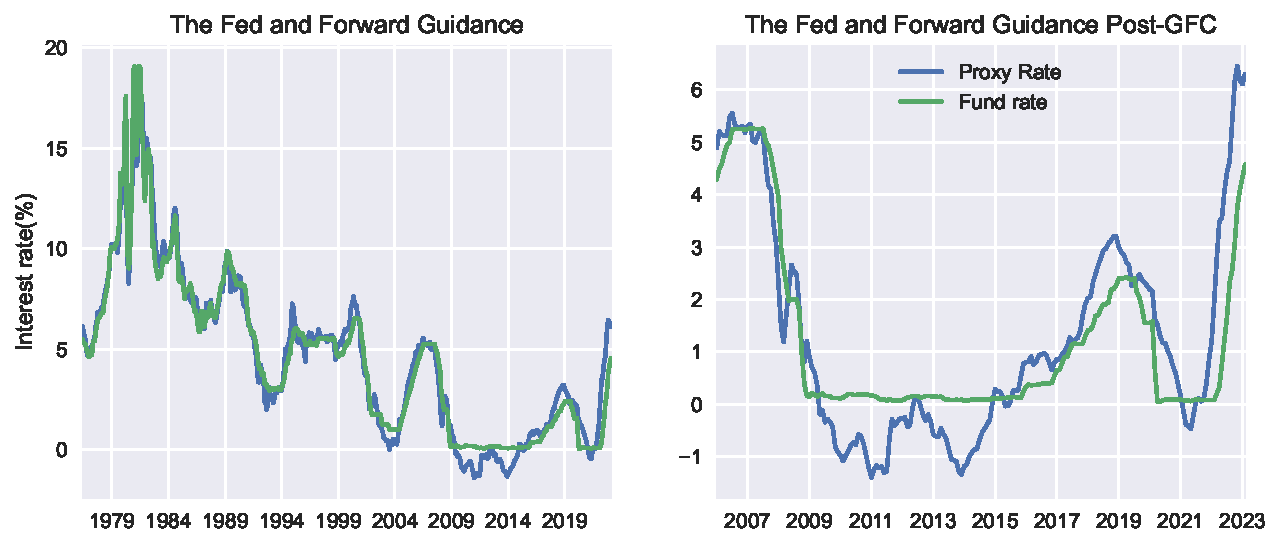
\includegraphics{Hawkish_Fed_files/figure-pdf/fig-1-output-1.pdf}

}

\caption{\label{fig-1}The Proxy and Policy Rate}

\end{figure}

The Fed has been criticized (including by respected
\href{https://www.lse.ac.uk/CFM/assets/pdf/CFM-Discussion-Papers-2022/CFMDP2022-09-Paper.pdf}{academics})
for acting too slowly to address inflation, but the truth is that they
began to tighten financial conditions well before the interest rate
hikes. In fact, they started eight months before the first hike in March
2022, and almost a year and a half after the pandemic shock
(Figure~\ref{fig-1}). This is important to note, because when the Fed
changed course, inflation was mostly driven by
\href{https://www.frbsf.org/economic-research/indicators-data/supply-and-demand-driven-pce-inflation/}{supply-side
factors}, such as supply chain disruptions and labor shortages. This
left less room for monetary policy to do much. However, the Fed clearly
began to change course before the pressure from the demand side on
inflation started to substantially pick up.

It's worth emphasizing that even prior to the Global Financial Crisis
(GFC), the proxy rate and the fund rate were not identical. Part of this
discrepancy can be attributed to the inevitable measurement errors
involved in calculating a statistical measure such as the proxy rate. Of
course, it's impossible to completely eliminate statistical errors, but
we can reasonably assume that most of the difference between the proxy
rate and the fund rate can be attributed to communication-related
factors.

This evidence makes it clear that the inclusion of forward guidance and
other unconventional tools has expanded the criteria by which the
monetary policy stance should be evaluated. It is now clear that the Fed
has become looser than it appears when stimulating the economy, and
tighter than the policy rate indicates when tightening. As a result, it
is becoming more important to get a better sense of the magnitude of the
non-conventional aspects of monetary policy. The following paragraphs
will examine this issue more closely.

\hypertarget{until-the-job-is-done}{%
\subsection{``Until the Job is Done''}\label{until-the-job-is-done}}

The difference between the proxy and policy rate shows the level of
interest rate implied by the Fed's forward guidance. Figure~\ref{fig-2}
shows exactly this. For example, at the peak of the proxy rate during
this monetary policy tightening cycle, the Fed added an extra 3\% to the
policy rate by just pointing what will be doing. This means that until
October 2022, the economy was effectively operating at an interest rate
level closer to 6\% than the official policy rate of 3\%\footnote{It is
  sometimes surprising to hear Fed officials (such as James B. Bullard)
  support their arguments for the appropriate policy rate by referring
  to the Taylor rule, without considering the effects of direct
  communication, including the signals that their analysis sends to the
  markets. But it is even more surprising that analysts, journalists,
  and strategists often perpetuate the flaws in their thinking.}. It was
only after October 2022 that the proxy rate start coming off, signaling
a less hawkish stance.

\begin{figure}

{\centering 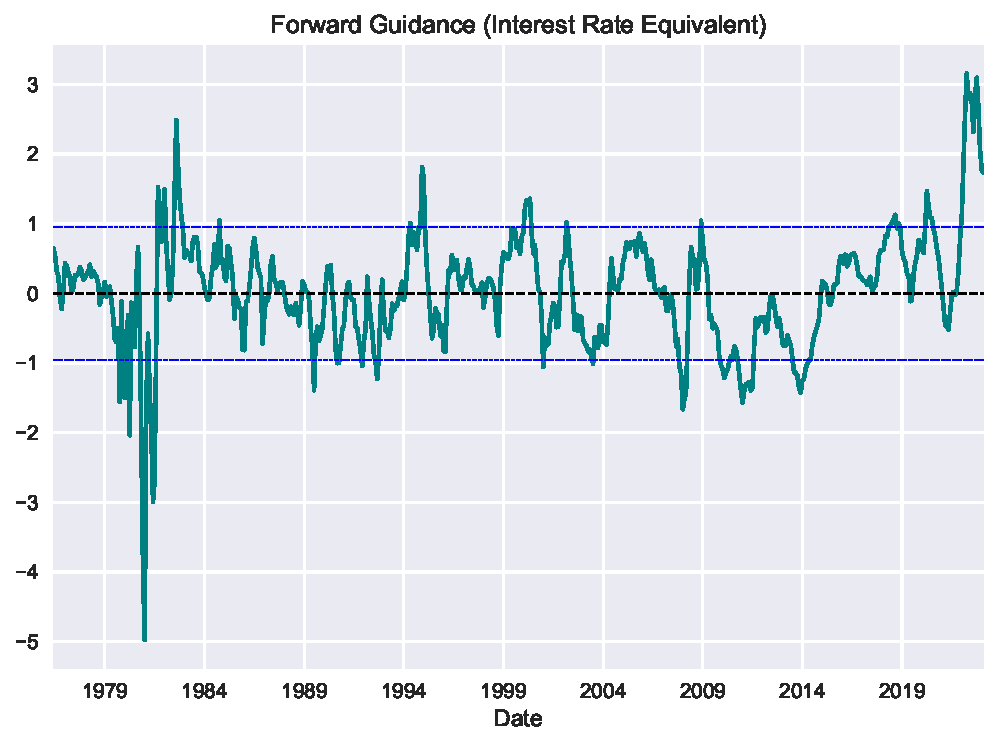
\includegraphics{Hawkish_Fed_files/figure-pdf/fig-2-output-1.pdf}

}

\caption{\label{fig-2}Interest Rates equivalent of Direct Communication}

\end{figure}

Fed's tone shift was mostly evident in Jay Powell's Jackson Hole speech
last August who declared ``the Federal Reserve must keep at it until the
job is done''. The US stock market slid sharply after Powell spoke, with
the benchmark S\&P 500 index falling 3.4 per cent, while the tech-heavy
Nasdaq Composite tumbled 3.9 per cent, recording the one biggest one-day
decline for both indices (outside sudden crashes).

To put things in perspective, in Figure~\ref{fig-3} I show the magnitude
of this and other messages since 2020 and compare the unconventional
part of the monetary policy to historical standards. The calculations
are still based on the distance between the proxy rate and the policy
rate. The left panel shows the average impact of communication-related
factors across all tightening episodes since mid-70s as identified by
the proxy rate. For the relevant periods, I have also filtered out the
direct impact of balance sheet changes\footnote{To filter out the direct
  impact of balance sheet changes, I controlled for the change in 10Y
  Treasuries. This may not completely capture the full impact, but it
  should be close. Only the first round of QE was strong enough.
  Subsequent rounds were less effective as markets anticipated the Fed's
  actions. That is the reason why Bernanke wanted more QE to offset
  these effects and compensate for the tight fiscal policy at the time.
  A classic study is the one by
  \href{https://www.nber.org/papers/w17555}{Krishnamurthy and
  Vissing-Jorgensen}.}. The right panel shows the distribution of the
interest rates implied by forward guidance across each
decades\footnote{For readers not familiar with box plots see this
  \href{https://en.wikipedia.org/wiki/Box_plot}{post}}.

\begin{figure}

{\centering 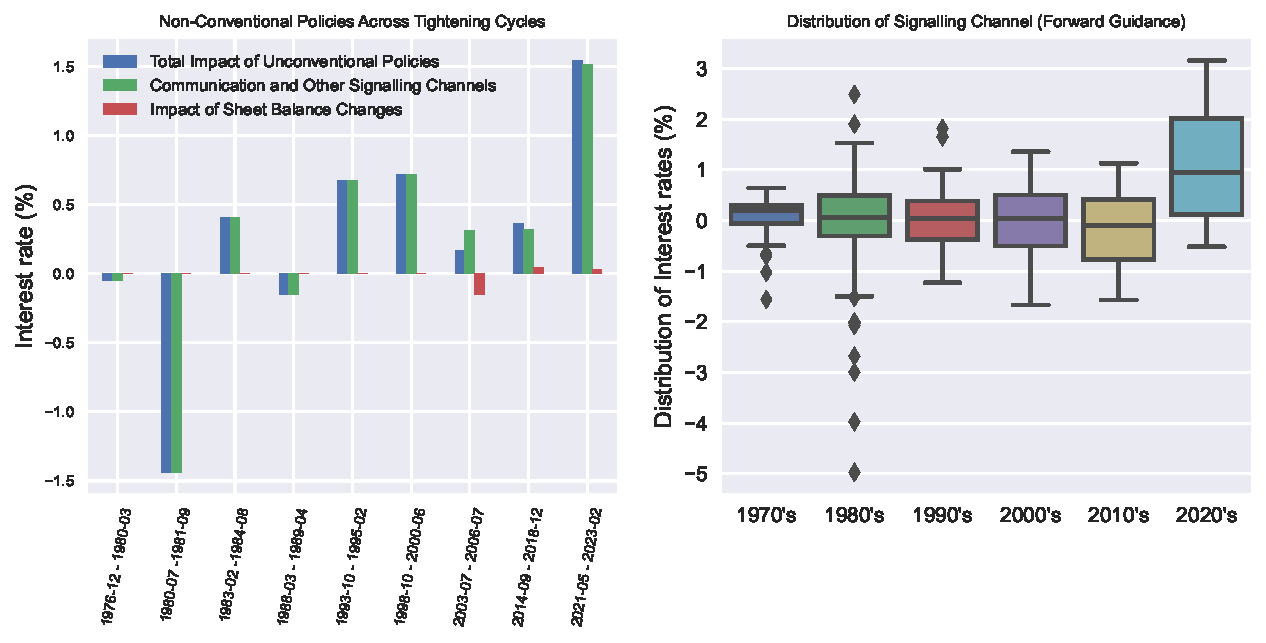
\includegraphics{Hawkish_Fed_files/figure-pdf/fig-3-output-1.pdf}

}

\caption{\label{fig-3}Monetary Policy Tightening Cycles}

\end{figure}

Ben Bernanke once said that ``monetary policy is 99\% words and 1\%
action.'' This was certainly true in the current tightening cycle, where
the Fed's words had an unprecedented impact. The Fed's communication and
signaling factors added (on average) an additional 1.5 percent of
interest rates hikes, which is three times more than the most aggressive
Fed of the past.

The credibility factor also played a role here. Before gaining the
``credibility medal'' the Fed struggled to convince the markets in the
first two tightening cycles in Figure 3, even though it raised rates
significantly. Things changed with Paul Volcker, but it wasn't until
forward guidance became part of the monetary policy transmission
mechanism that markets started taking the Fed seriously.

Another way to look at the impact of the Fed's messaging in recent years
is to look at the right panel of Figure~\ref{fig-3}, where I have
plotted the distribution of the impact of forward guidance (in terms of
interest rates). The Fed is now more likely to be seen as hawkish than
dovish, given its seriousness in fighting inflation and the fact that
markets still have faith in its words. This was not the case in the
1970s and 1980s. It is also worth noting that the formal incorporation
of forward guidance has managed to have a relatively even impact across
different economic conditions, indicating some ability to weigh the
balance of risks and fine-tune its words to the situation.

\hypertarget{the-implications-for-soft-landing}{%
\subsection{The implications for Soft
Landing}\label{the-implications-for-soft-landing}}

In the meantime, the Fed has carried out the swiftest policy rate
increase in the history of the United States. As I have briefly
discussed in a previous
\href{https://msh855.github.io/TheQuantEconomist/posts/fed_and_private_consumption/the_fed_and_private_consumption.html}{post},
the present interest rate level suggests that the impact on output is
likely to be just as significant. This implies that the response from
the Fed's end has been sufficiently forceful in all areas under its
\emph{direct} control. It's hard not to draw the conclusion that we are
presently experiencing the most hawkish monetary policy position in
recent US history, and its repercussions are just beginning to
materialize\footnote{We can discuss about the level of interest rates,
  but as I have explained in an earlier
  \href{https://msh855.github.io/TheQuantEconomist/posts/fed_and_private_consumption/the_fed_and_private_consumption.html}{post}
  I am very critical of the standard practice in using the distance of
  the policy rate relative to the neutral rates to indicate how neutral
  monetary policy is.}.

Does this mean that a
\href{https://www.investopedia.com/terms/s/softlanding.asp}{soft
landing} is off the table? That's a whole other discussion. But the
short answer is ``No''. In fact, the opposite is true. According to this
evidence, the Fed's actions are what kept a soft landing on the cards.
And, this shouldn't be surprising. Technically, only the Fed needs to
comply to a soft landing because of its mandate to balance maximum
employment and price stability. Other central banks don't have this
restriction\footnote{Although, they still care about unemployment to
  avoid overshooting or undershooting inflation.}.

Nevertheless, soft landing is still the holy grail of central banking.
\href{https://en.wikipedia.org/wiki/Rudi_Dornbusch}{R. Dornbusch}
famously said, ``\emph{No postwar recovery has died in bed of old
age---the Federal Reserve has murdered every one of them}''. The most
notable (and technically the only) soft landing in the most recent 16
business cycles occurred in 1994 under Alan Greenspan. Inflation was
rising rapidly in 1994, and Greenspan raised interest rates seven times
in the space of a year, bringing them up to 6\%. This was a significant
increase, but it did not cause a recession. In fact, the economy
continued to grow throughout 1994 and 1995. Why was it successful?
Economists will pick three main reasons:

\begin{itemize}
\tightlist
\item
  First, the economy was strong at the time, which helped to cushion the
  impact of the higher interest rates.
\item
  Second, Greenspan was able to communicate his intentions clearly to
  the public, which helped to reduce uncertainty.
\item
  Third, Greenspan was able to raise interest rates gradually, giving
  businesses and consumers time to adjust.
\end{itemize}

In Figure~\ref{fig-5}, I plotted this episode and compared it to the
current tightening cycle. I also added the ``Hard landing'' of Volcker
(which was essentially started by Burns and Miller) and the in-between
tightening cycle of 1999 to make the case clearer. Before the 1980s, any
comparisons are meaningless, as the Gold Standard was in place, there
was a substantially different monetary policy framework, and fiscal
dominance was the norm. I also ignored the tightening cycle that
preceded the Global Financial Crisis (for obvious reasons) and the
tightening cycle of 2018, as it was disrupted by the pandemic.

\begin{figure}

{\centering 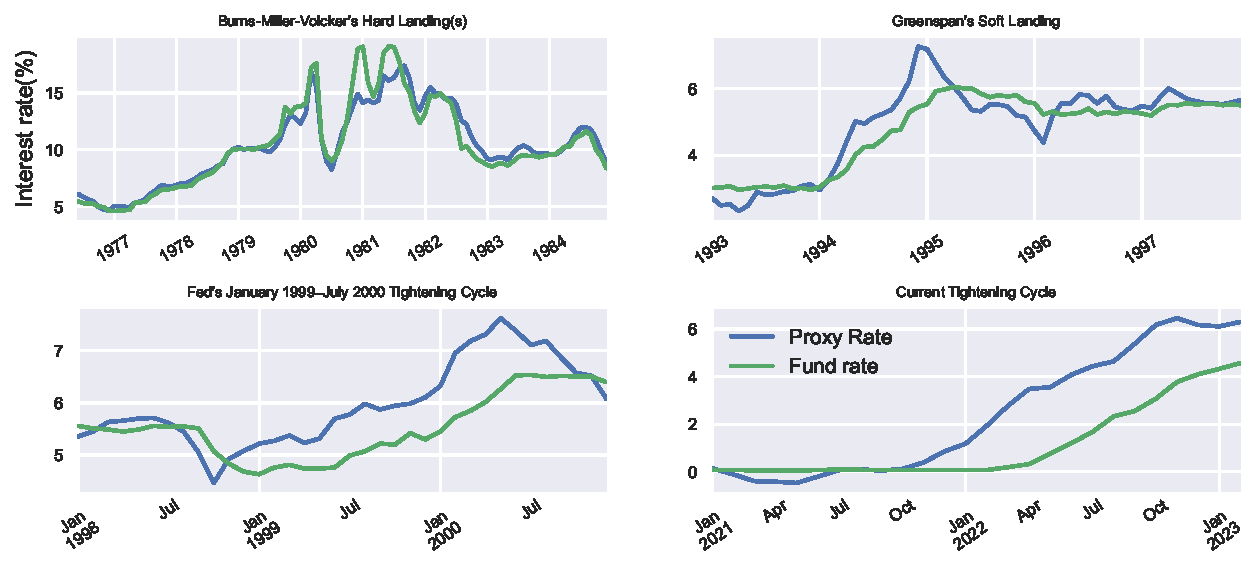
\includegraphics{Hawkish_Fed_files/figure-pdf/fig-5-output-1.pdf}

}

\caption{\label{fig-5}Monetary Policy Tightening Cycles}

\end{figure}

The Fed's reaction function under Greenspan and now is quite similar,
including making up for Friedman's ``long and variable lags.'' However,
unlike in the past, the use of unconventional tools allows the Fed to
adjust its policy more smoothly and early on, without raising the policy
rate. The three conditions that made Greenspan a legend continue to hold
in some reasonable sense. The dynamics are also similar to the
tightening cycle of 1999, which ended with the dot-com crash. However,
as the ``mini'' banking crash clearly demonstrated, the financial system
is much more resilient today. Of course, there are some factors that are
different between now and then, such as the starting level of inflation.
However, a full assessment of all these factors would require a whole
new discussion.

To conclude, a soft landing is primarily a fine-tuning exercise that is
difficult to achieve, almost identical if not as elusive as timing the
market. Based on the evidence here, the Fed has taken all necessary
steps to achieve this goal and some of the necessary conditions for a
soft landing are clearly met. But I do think that, overall, luck factors
are more important than they were in the past\footnote{I call ``luck
  factors'' the factors that central banks cannot fully control, such as
  consumer and business behavior. These behaviors are generally stable
  and predictable, but they can be disrupted by indirect or second-round
  effects of monetary policy. These indirect effects are what make the
  effects of monetary policy have ``long and variable lags.'' Supply
  shocks are also ``luck factors'' as are any other unanticipated
  shocks. In addition, a soft landing substantially depends on the pace
  at which central banks want to bring inflation down. A fast pace
  implies less chance of a soft landing, as it would require the real
  economy to be crashed. Too slow also reduces the chance of a soft
  landing, as there is a high chance that inflation expectations will
  become de-anchored and new unfavorable shocks will hit the system.}.



\end{document}
